\section{CSIRT aufbauen}

\subsection{Begriffe}

\subsubsection{CSIRT (Computer Security Incident Response Team)}
Ein \textit{CSIRT} ist ein Team von IT-Sicherheitsexperten, dessen Hauptaufgabe darin besteht, auf Computersicherheitsvorfälle zu reagieren. Es bietet die notwendigen Dienstleistungen an, um diese zu bearbeiten und die Betroffenen bei der Wiederherstellung nach Verstössen zu unterstützen.

\begin{itemize}
    \item Präziser, Free to use, ca. 19 Teams in CH
    \item CSIRT wird oft beim Besprechen der Aktivitäten verwendet
    \item CERT kommt gerne in den Teambezeichnungen vor
    \item NCSC (National Cyber Security Centre) ist ein verwendeter Betriff für ein \glqq nationales CSIRT\grqq
    \begin{itemize}
        \item Ein NCSC hat im Normalfall einen Auftrag vom Staat. Dieses kann mehr/anders sein, als von einem CSIRT erwartet
    \end{itemize}
\end{itemize}
 Wird oft als synonym verwendet zu \textit{CERT (Computer Emergency Response Team)}.

 \paragraph{Grundlagen eines CSIRT}
 \begin{itemize}
    \item Ein CSIRT ist eine Organisationseinheit
    \item Es bietet einem \underline{bestimmten} Personenkreis Dienstleistungen und Unterstützung an
    \item Es ist in der Verhütung, Erkennung, Behandlung und Reaktion auf Sicherheitsvorfälle involviert
    \item Es hat einen Auftrag
 \end{itemize}

\subsubsection{Formen eines CSIRT}
\paragraph{Internes Team}
\begin{itemize}
    \item Dediziertes Team innerhalb der Organisation
    \item Team besteht aus Personen, die nur fürs CSIRT arbeiten
    \item Typisch für grössere Organisationen, die sich ein dediziertes Team leisten können
\end{itemize}

\paragraph{Virtuelles Team}
\begin{itemize}
    \item Team besteht aus Personen, die in mehreren Teams arbeiten
    \item Typisch für kleinere Organisationen und solche, die einen Teil durch Dritte leisten lassen
\end{itemize}

\paragraph{Externes Team}
\begin{itemize}
    \item CSIRT Dritter als Dienstleistung beziehen
    \item \textbf{Achtung}: Internes Personal zwingend notwendig, mindestens in Form eines virtuellen Teams!
\end{itemize}

\subsubsection{SOC (Security Operations Center)}
\begin{itemize}
    \item Sammelt Aktivitäten und Ereignisse von Servern, Clients, Netzwerken etc.
    \item Fortlaufende, automatische Analyse dieser Aktivitäten auf verdächtiges Verhalte
    \item Verifikation der Auffälligkeit (wird Ereignissfall zum Vorfall oder bleibt es beim Ereignis)
    \item Eskalation zur Nachverfolgung/Lösung (→ Sicherheitsereignis/-vorfall)
    \item nicht nur Monitoring, sondern kann auch Zertifikate erstellen, Berechtigungen vergeben oder sogar ein \glqq halbes CSIRT\grqq{} ist
\end{itemize}

\paragraph{SOC-Betriebsmodell: Bereitstellungsmethode}
\begin{center}
    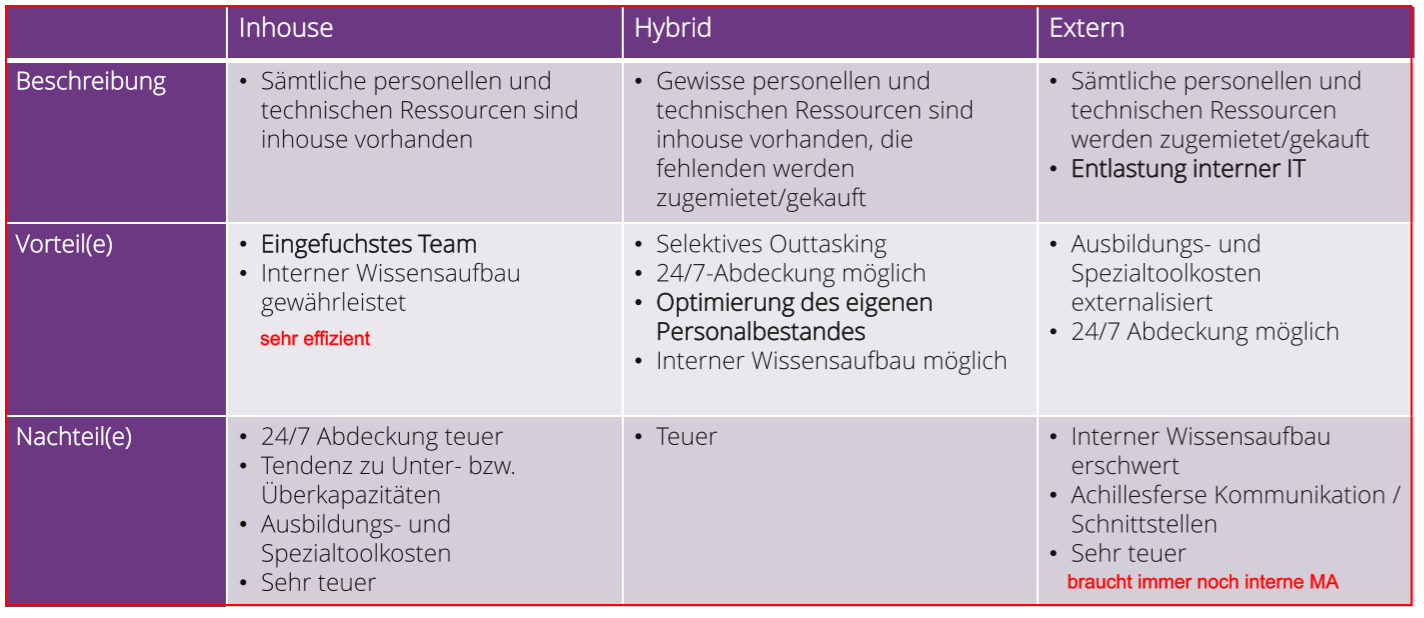
\includegraphics[width=1.0\linewidth]{04-csirt/03-soc_betriebsmodell}
\end{center}

\subsubsection{SIEM (Security Information and Event Management)}
\begin{itemize}
    \item IT-System (Software + Hardware) zur Sammlung von Systemverhaltensdaten und der automatischen Auswertung dieser
\end{itemize}

\subsubsection{MDR (Managed Detection \& Response)}
\begin{minipage}{0.4\linewidth}
    \paragraph{Detect}
    \begin{itemize}
        \item Standardwerte und –verhalten feststellen
        \item Abweichungen von der Norm erkennen
        \item Informationssicherheitsereignisse erkennen/entdecken
        \item Festlegen, wann ein Informationssicherheitsvorfall vorliegt
        \item Verwundbarkeitsscans \& Asset Überwachung
    \end{itemize}
    \vfill
    $ $
\end{minipage}
\begin{minipage}{0.6\linewidth}
    \paragraph{Respond}
    \begin{itemize}
        \item Informationssicherheitsereignisse analysieren
        \item Informationssicherheitsvorfall bewältigen
    \end{itemize}
\end{minipage}

\subsection{CSIRT Lifecycle}
\begin{center}
    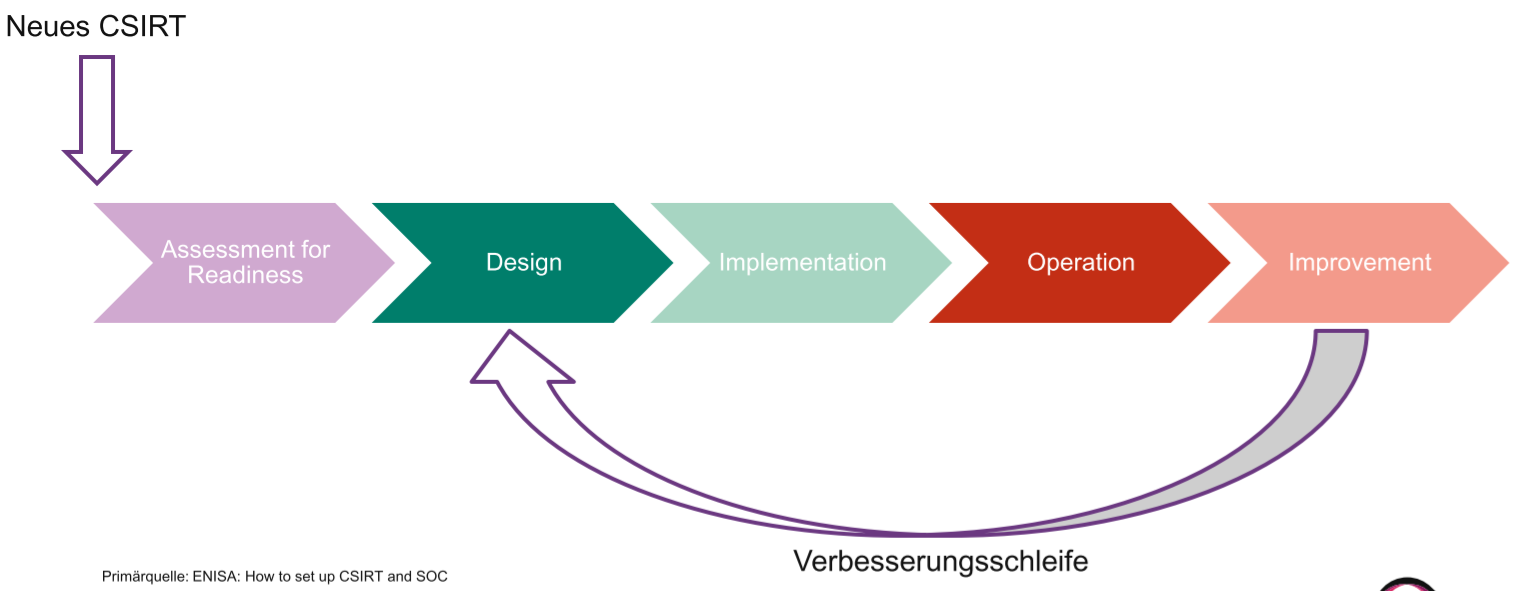
\includegraphics[width=1.0\linewidth]{04-csirt/01-csirt_lifecycle}
\end{center}

\textbf{\textcolor{red}{Verbesserungsschleife ist sehr wichtig $\rightarrow$ besser werden}}

\subsubsection{Assessment for Readiness}
\begin{minipage}{0.4\linewidth}
    \paragraph{Mandat}
    \begin{itemize}
        \item Was ist der Zweck des CSIRT?
        \item Wieso ist ein CSIRT notwendig?
        \item Welche Rechte und Pflichten hat das CSIRT?
    \end{itemize}
    \vfill
    $ $
\end{minipage}
\begin{minipage}{0.6\linewidth}
    \paragraph{Struktur}
    \begin{itemize}
        \item Wer finanziert das CSIRT?
        \item Wer ist für das CSIRT verantwortlich?
        \item Mit welchen Stellen/Organisationen/Abteilungen/… muss es interagieren?
    \end{itemize}
\end{minipage}

\paragraph{Ziel dieser Phase}
\begin{itemize}
    \item Grober Umsetzungsplan und Budget
    \item Anforderungen für die Design-Phase
    \begin{itemize}
        \item Mandat, Umsetzungsplan, Budget
        \item Rollen, Fähigkeiten, Ressourcen usw., die für die Design-Phase zur Verfügung stehen
    \end{itemize}
\end{itemize}

\subsubsection{Design}
\begin{itemize}
    \item CSIRT Dienstleistungen definieren
    \item CSIRT Prozesse und Abläufe definieren
    \item Organisationsstruktur und die Fähigkeiten der CSIRT Rollen
    \item Definition des notwendigen Wissens fürs CSIRT und Weiterbildungen
    \item Anforderungen an die Büroräumlichkeiten und deren Verteilung, Technologien
    \item Angestrebte interne und externe Partnerschaften
    \item Informationssicherheitsmanagement
    \item Anforderungen und Ziele der Implementation-Phase
\end{itemize}

\subsubsection{Implementation}
\begin{itemize}
    \item Notwendiges Personal anstellen oder ins CSIRT integrieren
    \item Bei Bedarf die Mitarbeitenden gemäss Profilanforderungen weiterbilden
    \item Umsetzung der Anforderung an die Räumlichkeiten, Technologien, Prozesse, ans Informationssicherheitsmanagement etc. aus der \textit{Design}-Phase
    \item CSIRT Prozesse trainieren
    \item Kontaktaufnahme und Vernetzung mit internen/externen Partnern
\end{itemize}

\paragraph{Was für Dokumente/ Richtlinien sollte ein CSIRT haben?}
Diese sollen sicherstellen, dass Information zu Vorfällen, Schwachstellen, Artefakten etc. geschützt sind.\\

\begin{minipage}{0.4\linewidth}
    \begin{itemize}
        \item Klassifizierung von Informationen
        \item Schutz von Informationen
        \item Aufbewahrung von Informationen
        \item Vernichtung von Informationen
        \item Weitergabe von Informationen
    \end{itemize}
    \vfill
    $ $
\end{minipage}
\begin{minipage}{0.6\linewidth}
    \begin{itemize}
        \item Zugang zu Informationen
        \item Nutzungsreglement für die CSIRT-Systeme
        \item Definition / Klassifikation / Kategorisierung von Ereignissen und Vorfällen
        \item Behandlung von Vorfällen
        \item Zusammenarbeit mit anderen Teams
    \end{itemize}
\end{minipage}

\subsubsection{Operations}
\begin{itemize}
    \item Fortlaufend die Arbeit überwachen und messen (Stichwort: Key Performance Indicators (KPI))
    \item Regelmässige Qualitätsprüfung und Erfüllung der Vorgaben prüfen
    \item Weiterentwicklungsmöglichkeiten identifizieren und sammeln
    \item Und die eigentliche CSIRT-Arbeit leisten
\end{itemize}

\subsubsection{Improvement}
\begin{itemize}
    \item Vorschläge für Verbesserungen sammeln
    \item Vorgehen und Anforderungen für die Entwicklung der Verbesserungen (\textit{Design}-Phase) festlegen
    \item Notwendige Ressourcen (z. B. Budget) organisieren, damit die \textit{Design}-Phase starten kann
\end{itemize}

\subsection{CSIRT-Dienste}

\subsubsection{CSIRT Service Areas}
\begin{center}
    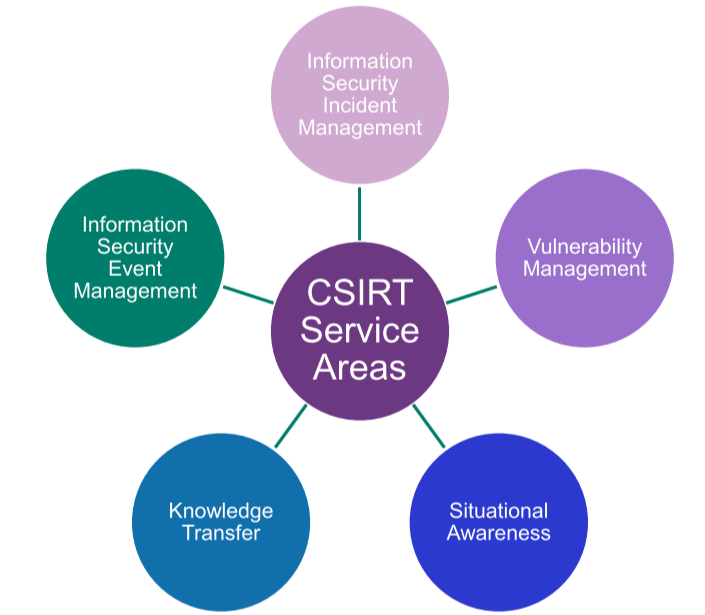
\includegraphics[width=0.5\linewidth]{04-csirt/02-csirt_service_areas}
\end{center}

\paragraph{Information Security Event Management}
\begin{itemize}
    \item Daten aus Ereignisquellen sammeln, korrelieren, anreichern, auswerten und mögliche Informationssicherheitsereignisse identifizieren
    \item Fortlaufend Daten aus Ereignisquellen sammeln
    \item Ereignisdaten durch zusätzliche Informationen anreichern (z. B. Kontext, Threat Intelligence)
    \item Gesammelte Daten analysieren und verdächtige Muster identifizieren und möglichst alles automatisieren
    \item Nicht nur «Logs», sondern auch Netzwerkverkehr (z. B. NetFlow), Meldungen von IDS, Meldungen von Externen etc.
\end{itemize}

\paragraph{Information Security Incident Management}
\begin{itemize}
    \item Zentrales Element der Arbeit des CSIRT
    \item Beinhaltet das, was wir aus den Incident Response Prozessen bereits gelernt haben
    \item Schwerpunkte im CSIRT Service Framework
    \begin{itemize}
        \item \textit{Vorfälle koordinieren}: Fluss und Weitergabe von Informationen zum Vorfall sicherstellen
        \item \textit{Krisenmanagement}: Unterstützung, wenn ein Vorfall zur Krise für die Organisation wird
    \end{itemize}
\end{itemize}

\paragraph{Vulnerability Management}
\begin{itemize}
    \item Die hier erbrachten Dienste sind \underline{stark von der Organisation abhängig}
    \item \glqq Klassische\grqq{} Vulnerability Management
    \begin{itemize}
        \item Schwachstellen entdecken (fortlaufend und/oder auch während einem Vorfall)
        \item Schwachstellenberichte entgegennehmen \& auf Schwachstellen reagieren
    \end{itemize}
    \item Kann aber auch noch enthalten:
    \begin{itemize}
        \item Bisher unbekannte Schwachstellen suchen
        \item Mit involvierten Parteien koordinieren: Wissensaustausch, z. B. im Rahmen einer koordinierten Offenlegung von Schwachtellen
        \item Informationen zum Vermeiden und Auffinden und Massnahmeempfehlungen
    \end{itemize}
\end{itemize}

\paragraph{Situational Awareness}
\begin{itemize}
    \item Verstehen was in und um die Aktivitäten und Themen des CSIRT geschieht
    \begin{itemize}
        \item Sowohl interne als auch externe Informationsquellen
        \item Sowohl technische, organisatorische und weitere nicht-technische Informationen
    \end{itemize}
    \item Beispiele
    \begin{itemize}
        \item Übersicht aller (kritischen) Assets, dafür verantwortliche Personen/Rollen, deren normales Verhalten, Kritikalität für die Organisation etc.
        \item Beobachtung relevanter Medien, anderer CSIRTs/PSIRTs, technologische Entwicklungen etc.
        \item Beobachtung interner Veränderungen und organisatorischer Aktivitäten innerhalb der Organisation
        \item Relevante Daten fürs Security Event Management sammeln
    \end{itemize}
    \item Unterstützt andere CSIRT Services (Security Event Management, Incident Management, Knowledge Transfer)
    \item Kann auch eine Quelle zur Bewertung neuer / anstehender Gefahren dienen
    \item Kann auch juristische, politische, geopolitische Themen abdecken
\end{itemize}

\paragraph{Knowledge Transfer}
\begin{itemize}
    \item CSIRTs haben einen einmaligen Einblick in die Informationssicherheit
    \begin{itemize}
        \item Beschäftigen sich im Normalfall mit der aktuellen Bedrohungslage
        \item Haben Einblick in Angriffe gegen die Organisation
        \item Tauschen sich mit anderen Organisationen/Teams aus und erhalten breiten Einblick in aktuelle Themen
        \item Sind meistens gut vernetzt innerhalb der Organisation und haben einen vielseitigen Einblick
    \end{itemize}
    \item All dies ist ideal für die Weitergabe dieses Wissens zur Steigerung der Informationssicherheit
    \begin{itemize}
        \item Bewusstsein fürs Thema steigern (Awareness Training/Building)
        \item Aus- und Weiterbildung für andere Teams anbieten (z. B. richtiges Verhalten im Ernstfall)
        \item Übungen und Simulationen durchführen
        \item Sich in Richtlinien, Prozessen, Projekten und anderen organisatorischen Aktivitäten einbringen
    \end{itemize}
\end{itemize}

